\documentclass[12pt,ignorenonframetext,compress]{beamer}
\usetheme{Warsaw}
\setbeamertemplate{caption}[numbered]
\setbeamertemplate{caption label separator}{:}
\setbeamercolor{caption name}{fg=normal text.fg}
\usepackage{amssymb,amsmath}
\usepackage{ifxetex,ifluatex}
\usepackage{fixltx2e} % provides \textsubscript
\usepackage{lmodern}
\ifxetex
  \usepackage{fontspec,xltxtra,xunicode}
  \defaultfontfeatures{Mapping=tex-text,Scale=MatchLowercase}
  \newcommand{\euro}{€}
\else
  \ifluatex
    \usepackage{fontspec}
    \defaultfontfeatures{Mapping=tex-text,Scale=MatchLowercase}
    \newcommand{\euro}{€}
  \else
    \usepackage[T1]{fontenc}
    \usepackage[utf8]{inputenc}
      \fi
\fi
% use upquote if available, for straight quotes in verbatim environments
\IfFileExists{upquote.sty}{\usepackage{upquote}}{}
% use microtype if available
\IfFileExists{microtype.sty}{\usepackage{microtype}}{}
\usepackage{url}

% Comment these out if you don't want a slide with just the
% part/section/subsection/subsubsection title:
\AtBeginPart{
  \let\insertpartnumber\relax
  \let\partname\relax
  \frame{\partpage}
}
\AtBeginSection{
  \let\insertsectionnumber\relax
  \let\sectionname\relax
  \frame{\sectionpage}
}
\AtBeginSubsection{
  \let\insertsubsectionnumber\relax
  \let\subsectionname\relax
  \frame{\subsectionpage}
}

\setlength{\parindent}{0pt}
\setlength{\parskip}{6pt plus 2pt minus 1pt}
\setlength{\emergencystretch}{3em}  % prevent overfull lines
\setcounter{secnumdepth}{0}

\definecolor{links}{HTML}{2A1B81}
\hypersetup{colorlinks,linkcolor=,urlcolor=links}

\title{R, Rcpp and Parallel Computing}
\subtitle{Notes from our Rcpp Experience}
\author{Dirk Eddelbuettel and JJ Allaire}
\date{Jan 26-27, 2015\newline Workshop for Distributed Computing in R}

\begin{document}
\frame{\titlepage}

\section{Intro}\label{intro}

\begin{frame}{One View on Parallel Computing}

\begin{quote}
The whole ``let's parallelize'' thing is a huge waste of everybody's
time. There's this huge body of ``knowledge'' that parallel is somehow
more efficient, and that whole huge body is pure and utter garbage. Big
caches are efficient. Parallel stupid small cores without caches are
horrible unless you have a very specific load that is hugely regular (ie
graphics).

{[}\ldots{}{]}

Give it up. The whole ``parallel computing is the future'' is a bunch of
crock.
\end{quote}

\href{http://www.realworldtech.com/forum/?threadid=146066\&curpostid=146227}{Linus
Torvalds, Dec 2014}

\end{frame}

\begin{frame}{Another View on Big Data}

\begin{figure}
\begin{center}
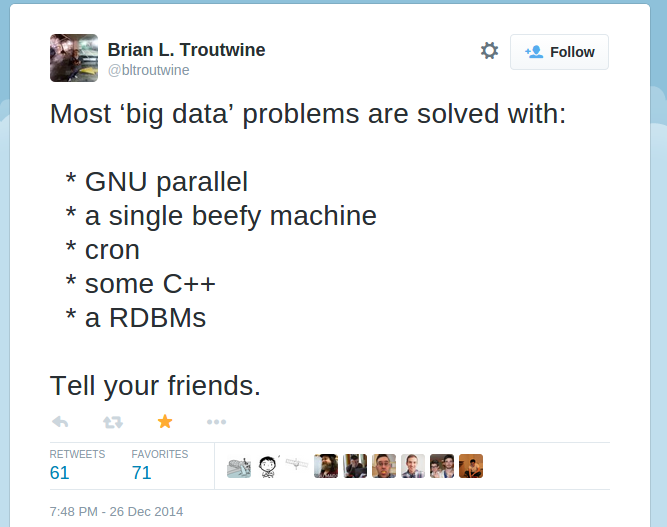
\includegraphics[width=\textwidth,height=0.8\textheight,keepaspectratio]{images/big-data-big-machine-tweet.png}
\end{center}
\end{figure}

\end{frame}

\section{R}\label{r}

\begin{frame}{CRAN Task View on HPC}

\framesubtitle{Lots of existing work to draw from}

\begin{itemize}
\itemsep1pt\parskip0pt\parsep0pt
\item
  Package snow by Tierney et al a trailblazer
\item
  Package Rmpi equally important
\item
  Packages multicore nee parallel help Windows (l)users
\item
  Hundreds of applications
\item
  It just works for \emph{data parallel} tasks
\end{itemize}

\url{http://cran.r-project.org/web/views/HighPerformanceComputing.html}

\end{frame}

\begin{frame}{Rcpp: Early Days}

In the fairly early days of Rcpp, we also put out RInside as a simple
C++ class wrapper around the R-embedding API.

It got one clever patch taking this (ie: R wrapped in C++ with its own
\texttt{main()} and sticking it into MPI.

\end{frame}

\begin{frame}{Rcpp: More recently}

Rcpp has gotten fairly easy to use.

OpenMP is easy to use and widely supported (on suitable OS / compiler
combinations).

So we added support. Use not as wide-spread. Errors have commonality:
calling back into R.

\end{frame}

\begin{frame}{RcppParallel}

Easy-to-use-wrapper around Intel TBB (and TinyThreads where no TBB)

Users still attempt to use R objects\ldots{}

\end{frame}

\end{document}
